%----------------------------------------------------------------------------------------
%	CHAPTER 1
%----------------------------------------------------------------------------------------

\chapter{La surveillance de masse : une histoire de programmes}
\label{ch:programmes}

% ~\vfill
% \begin{doublespace}
% \noindent\fontsize{18}{22}\selectfont\itshape
% \nohyphenation
% \openepigraph{<< They who can give up essential liberty to obtain a little
% temporary safety, deserve neither liberty nor safety. >>}{-- Benjamin Franklin}
% \end{doublespace}
% \vfill
% \vfill

Comme il fut mentionné dans l'introduction, la surveillance généralisée est
permise à un niveau industriel à travers l'existence de programmes, aux bases
légales diverses, ayant chacun un but précis. Ces programmes fonctionnent (au
moins pour le cas des \EUA) comme des centaines de rouages permettant de faire
tourner la grande machine du renseignement.\newline

Seront présentés ici les programmes de surveillance qui ont fait parler d'eux
récemment (et moins récemment) via les révélations de Snowden, c'est à dire les
programmes américains et les différents programmes européens.

%------------------------------------------------

\newpage
\section{Le programme global des
\EUA}

\newthought{Le premier programme} connu pour avoir été massif dans ses
interceptions est ECHELON. Comme nous l'avons vu en introduction ce dernier fut
révélé en 1988 par un journaliste d'investigation spécialisé dans les services
de renseignements, mais son origine remonte jusqu'au traité UKUSA signé en 1946.
Les autres membres de Five Eyes ne rejoignirent ces deux pays qu'au cours des
années 1980, assurant ainsi une couverture globale des interceptions.

\begin{figure}
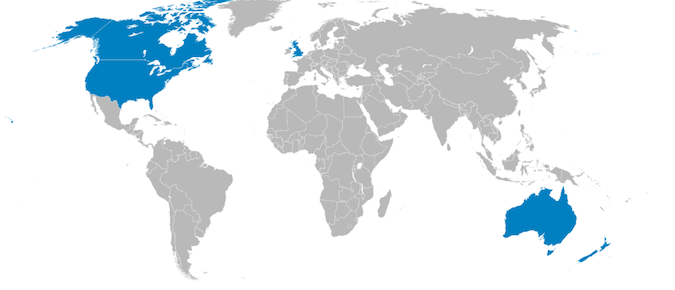
\includegraphics{fiveeyes.png}
\caption[Cartes de pays membres des Five Eyes][6pt]{Cartes de pays membres des
Fives eyes.}
\label{fig:carte}
\end{figure}

\newthought{Ce n'est qu'à} la fin des années 1960\autocite{ZDNET} qu'ECHELON fut
vraiment développé, lors des lancements des premiers satellites Intelsat. La
NSA\footnote{National Security Agency, l'agence chargée de la collecte des
informations électromagnétiques aux \EUA} et le GCHQ\footnote{Government
Communications Headquarters, le pendant britannique de la NSA} avaient besoin
d'accéder aux communications passées sur ces satellites, et décidèrent
donc de développer un réseau de stations d'écoutes terrestres, leur permettant
ainsi d'intercepter toutes les communications. Ainsi naquit ECHELON tel qu'on le
connaît encore aujourd'hui.

\newthought{Le programme s'est} renforcé au fur et à mesure des années, avec de
nouvelles stations, une orientation vers des interceptions sur fibre optique,
etc. Actuellement, il y aurait une quinzaine de stations d'écoutes réparties
dans le monde, selon un document de Snowden datant de 2012\autocite{Stations}.

\vspace{0.7cm}
\begin{figure}
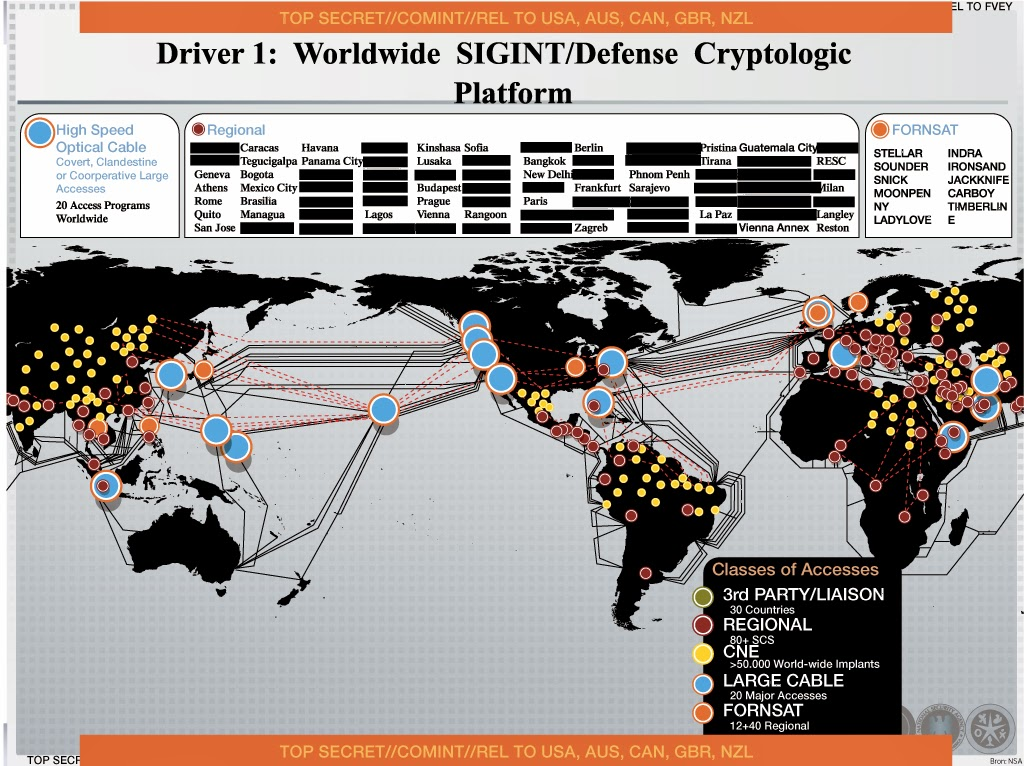
\includegraphics{carte.jpg}
\caption[Carte des stations d'interceptions][6pt]{Les points oranges
représentent les stations d'interceptions satellites.}
\label{fig:stations}
\end{figure}

\newthought{Comme le montre} la figure \ref{fig:stations}, les écoutes
concernent aussi maintenant les câbles sous-marins (contenant des fibres optiques) par
lesquels transitent 99\% des communications mondiales. 

\newthought{La NSA opère} également toute une myriade de programmes de
renseignement, afin de donner du sens aux données recueillies par les stations.
Du temps d'ECHELON, cela consistait en de gigantesques dictionnaires contenant
des mots-clés, que les supercalculateurs en charge de l'analyse pouvaient
isoler.

\newthought{Les documents de} Snowden ont permis de mettre à jour les détails
techniques des nouveaux programmes, dont les plus connus sont :

\subsection{PRISM}
\newthought{Le programme qui} a reçu le plus d'attention médiatique
lorsque les premiers documents de Snowden ont commencé à être révélés au public,
et certainement à juste titre, puisque le trafic généré par ce programme
représente 91\% du trafic de la NSA\autocite{WP91}. Les données proviennent
exclusivement des grandes entreprises du Web américaines (Google, Facebook,
Apple, etc) via l'utilisation de sélecteurs (des mots-clés, ou des requêtes
initiées par des analystes) qui vont aller chercher les informations quasiment
automatiquement.

\newthought{Ces révélations sur} les accès quasi-directs que possède la NSA sur
les serveurs des géants du Web furent très mal accueillies par ces derniers, qui
ont riposté en activant le chiffrement des communications sur leurs flux
internes\autocite{WPGoogle}, mettant à mal tout le dispositif clandestin. Il n'en
reste pas moins possible de passer par la voie légale pour obtenir les mêmes
données.

\newthought{En effet,} il est bon de rappeler brièvement que ces programmes ont
tous une base légale, à travers le FISA\footnote{Foreign Intelligence
Surveillance Act}. Ce texte, voté par le Congrès, décrit les modalités de
surveillance des citoyens \emph{étrangers}, impliquant que ces écoutes, ces
collectes et ces analyses en masse sont légalement permises. Elles n'ont pas
été remises en cause depuis l'instauration du Patriot Act en réaction aux attentats du 11 Septembre 2001.
Ce n'est que récemment (et suite aux révélations de Snowden) que ces programmes
et les pouvoirs qui leurs sont accordés furent remis en question.

\subsection{XKeyScore}
\newthought{L'un des programme} les plus mal connu, malgré les
documents publiés, mais également un des plus effrayants, de par l'ampleur de
son rayon d'action. 

\newthought{Il permettrait,} selon Glenn Greenwald, le journaliste qui a
interviewé Snowden et récupéré ses documents de <<~\ldots lire n'importe quel
courriel désiré, écouter n'importe quel appel téléphonique, historique de
navigation Web, documents Word. Et tout cela est fait sans demander à une cour,
sans demander l'approbation d'un superviseur pour cette part
d'analyse.~>>\autocite{GGW}

\newthought{Ce n'est pas} sans poser problème, puisqu'effectivement, ce dernier
ne semble pas avoir besoin de l'approbation de la FISC\footnote{Foreign
Intelligence Surveillance Court} pour les requêtes qui lui sont
fournies\autocite{Kimery}, contrairement au programme qui le précédait.

\subsection{Bullrun}

\newthought{C'est actuellement le} programme le plus cher de la NSA, avec un
coût total depuis son lancement, il y a dix ans, estimé à 800 millions
d'euros\autocite{bullrun} (par comparaison, PRISM ne coûte << que >> 20 millions
d'euros par an\ldots).
Sa fonctionnalité première semble être le décryptage de fichiers et de flux
chiffrés que l'Agence met de côté lorsqu'elle les intercepte. 

\newthought{Il semblerait aussi} qu'une autre facette de ce programme soit non
plus de l'ordre de la technique, mais dans la manipulation des standards de
chiffrement. En effet, il semble que la NSA ait poussé, au sein des instances
internationales en charge de la standardisation des méthodes de chiffrement, des
protocoles et des algorithmes qu'elle savait pouvoir casser\autocite{NYTenc} ou dans
lesquels elle avait délibérement inséré des portes dérobées.

\subsection{Dishfire}

\newthought{Ce programme est} actuellement opéré en partenariat avec le GCHQ
anglais. Il est spécialisé dans la collecte de messages textes (SMS) et dans la
géo-localisation de ces messages, la collecte de cartes de données
électroniques, des transactions de cartes de crédit circulant sans chiffrement sur le réseau,
les alertes d'appels manqués, les répondeurs, etc.

\newthought{Des aveux même} des analystes de la NSA et du GCHQ lors de la
présentation interne de ce programme, ce dernier collecte << à peu près tout ce
qu'il peut, donc vous pourriez voir des SMS de personnes qui ne sont pas visées
par vos requêtes. >>\autocite{Guardian}.

\newthought{Le gros avantage} de ce système est qu'il est possible de venir y
fouiller à posteriori. Lorsqu'une nouvelle cible est rentrée dans la base de
données, il est ainsi possible de retrouver ses anciens SMS et positions
géo-localisées afin d'affiner le profil.

\subsection{Upstream}

\newthought{Là où PRISM} pouvait être décrit comme << collecter tout ce qu'il
peut être collecté sur les réseaux sociaux >>, Upstream peut être décrit comme
<< collecter tout ce qu'on peut sur tout le reste >>. Contrairement à PRISM qui
est un programme autonome, Upstream se compose de multiples sous-programmes
(dont certains se composent eux-même de sous-programmes, il faut arriver à
suivre\ldots) :

\begin{itemize}
  \item FAIRVIEW : le programme chapeautant les trois autres.
  \item BLARNEY : se concentre sur la collecte de meta-données sur le réseau
  d'AT\&T\footnote{Grand opérateur de téléphonie américaine.}
  \item STORMBREW : se concentre sur les interceptions au niveau de l'opérateur
  Verizon.
  \item OAKSTAR : regroupement de 8 sous programmes, chacun spécialisé dans
  l'interception de méta-données dans une partie du monde.
\end{itemize}

\newthought{Selon les officiels}, cette collecte génère un flux très important
de données, et plusieurs filtres sont appliqués aux données collectées : les
opérateurs (AT\&T, Verizon, etc) font un premier filtre, en essayant de
supprimer au maximum les communications comprenant des citoyens américains.
Les communications restantes sont ensuite passées dans des sélecteurs (adresses
IP, numéros de téléphone, adresses mail, etc) afin d'en faire ressortir des
résultats. Le reste des données Internet peut ensuite être copié et utilisé à
travers XKeyScore pour des recherches futures.


\newthought{Tout ces programmes} ne sont que les plus gros exemples qui ont pu
être tirés des documents de Snowden. Il en existe encore beaucoup d'autres
(BoundLess Informant, RAGTIME, MAINWAY, MonsterMind, MYSTIC, TrailBlazer puis
Turbulence, MARINA, Dropmire pour les ambassades, Stateroom, etc), opérés par
la NSA seule ou bien en partenariat avec d'autres agences comme le GCHQ ou le
BND.

\vspace{0.8cm}
\begin{figure}
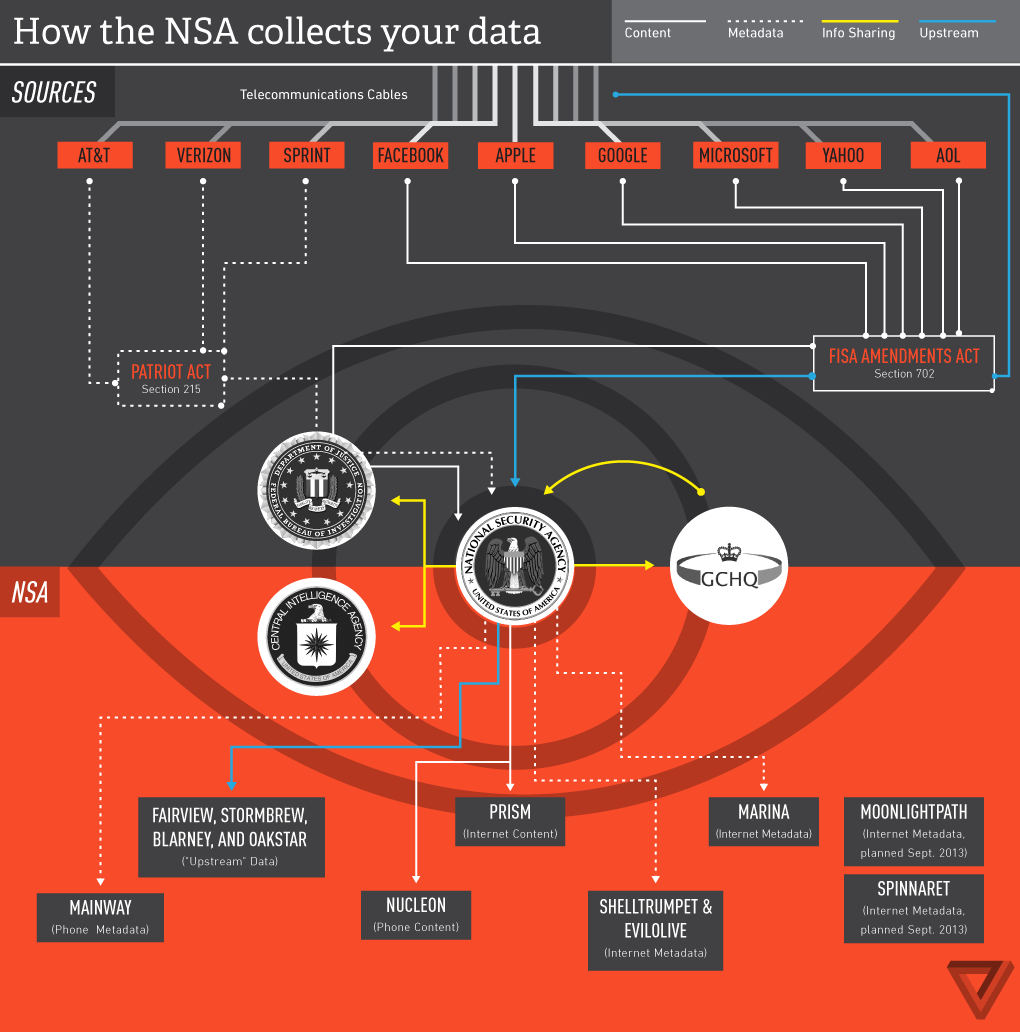
\includegraphics{flow.png}
\caption[Infographie résumant les différents programmes de
surveillance américains][6pt]{Résumé des différents programmes de collecte de
données de la NSA.}
\label{fig:infographie}
\end{figure}
\newpage
\newpage
\section{Les programmes en Europe : introduction}
\newthought{Nous l'avons vu,} les agences américaines sont assez prolifiques en
matière de programmes de surveillance (avec un budget estimé à 10.3 milliards de
dollars pour la NSA\autocite{budget}, en même temps\ldots), mais nous allons voir
que les pays européens ne sont pas en reste, avec notamment trois grands compétiteurs sur ce
créneau, le Royaume-Uni, l'Allemagne, et la France.

\section{Le Royaume-Uni et le GCHQ}

\newthought{C'est LE champion} européen de la surveillance électronique de
masse. Le Royaume-Uni a une longue tradition dans le domaine du chiffre, il
n'est donc pas surprenant de voir les Britanniques très en avance dans ce
domaine. Leur partenariat historique avec les \EUA~en font les acteurs
désignés pour mener des projets communs avec la NSA, comme nous allons le voir.

\newthought{Les plus gros} programmes britanniques sont les suivant :

\subsection{Tempora}

\newthought{Mis en place} en 2008, ce programme d'interceptions des
communications transitant par fibres optiques est le plus gros programme
britannique en matière d'écoute et de renseignement électromagnétique.

\newthought{Encore maintenant,} et malgré la publication de divers documents
récupérés par Snowden, des doutes subsistent quant aux détails de fonctionnement
de ce programme. Par exemple, on ne sait pas si les différents opérateurs
propriétaires des fibres optiques mises sur écoutes sont parties prenantes de ce
dispositif (il existe de forts soupçons à l'encontre de BT\footnote{British
Telecom}, qui collabore déjà avec le GCHQ dans d'autres programmes) ou s'ils
sont des victimes forcées des pratiques de services de renseignement.

\newthought{Egalement, nous} ne savons actuellement pas quelles sont les
quantités de données et méta-données collectées, ni si le programme fait la
différence entre les données issues des cibles des services et celles des
citoyens ordinaires. Le Guardian croit savoir\autocite{Tempora} que le programme ne
fait pas de différence, ce qui pose de sérieuses questions quant à la légalité
de ce programme, puisqu'il n'y a techniquement aucun moyen de différencier de
façon fiable les communications de ressortissants britanniques et celles des
étrangers, et que l'écoute des premiers n'est pas encadrée par les mêmes lois
que l'écoute des seconds. 

\newthought{Dans tous les} cas, les données recueillies par ce programme sont
échangées avec la NSA dans le cadre des accords bilatéraux qui ont cours entre
les deux agences de renseignement, ce qui permet à chacune de s'affranchir des
limitations juridiques que leur imposent les lois les encadrant. Le GCHQ peut
récupérer des informations et des méta-données sur les citoyens américains,
chose que ne peut pas faire la NSA légalement, et les transmettre à cette
dernière, et inversement\autocite{echange}. Cela permet aux deux agences d'espionner
leurs ressortissants tout en s'affranchissant du contrôle des instances
judiciaires de leurs pays respectifs, ce qui est plus que discutable sur le plan
de l'éthique.

\subsection{MUSCULAR}

\newthought{MUSCULAR est le} nom du programme mis sur pied par le GCHQ afin de
pénétrer les réseaux internes de deux entreprises américaines, Google et Yahoo!.
D'un strict point de vue technique, le programme tirait parti du manque de
sécurisation des-dits réseaux\autocite{echange}\autocite{Yahoo} (où les responsables de
la sécurité ont très mal pris la nouvelle, sachant qu'ils étaient déjà obligés de collaborer
dans le cadre de PRISM avec les autorités\ldots)

\newthought{Ce programme collecte} apparemment beaucoup plus de méta-données que
ne le fait PRISM (environ deux fois plus\autocite{echange}), ce qui été un défi
technique pour la NSA (XKeyScore se << nourrissant >> de ces données en plus de
celles de PRISM, il a fallu re-dimensionner une partie de l'architecture).

\subsection{Squeaky Dolphin}

\newthought{C'est le premier} programme qui ne sert pas à récolter des données
sur des individus. En effet, celui-ci est dédié à l'analyse des tendances sur
les réseaux sociaux, notamment via le suivi des données issues des boutons
<<~J'aime~>> de Facebook (données qui sont depuis cette révélation
chiffrées\autocite{fbenc}) ainsi que des données statistiques des vidéos vues sur
Youtube, des visites faites sur les blogs de la plate-forme Blogspot (propriété
de Google), ainsi que des données disponibles sur Twitter.

\newpage
\subsection{Optic Nerve}

\newthought{Programme un peu} singulier par son aspect très ouvert, Optic Nerve
s'intéresse très spécifiquement aux conversations par webcam des utilisateurs de
la messagerie Yahoo!\autocite{yahoocam}, sans chercher précisément des cibles
pré-enregistrées.

\newthought{Le programme est} supposé avoir capturé des millions d'images, à
raison de cinq images par seconde\autocite{latribune}, dont de nombreuses images à
caractère sexuel ou pornographique. Cela a permis au GCHQ de tester et de
peaufiner des algorithmes de reconnaissance faciale.

\newthought{A travers ces} quelques exemples, nous voyons bien que la
Grande-Bretagne n'est pas en reste en matière de surveillance de masse. Le liens
de coopération privilégiée tissés avec la NSA lui assure un accès quasiment
illimité à XKeyScore et une grande marge de manoeuvre dans la mise en place de
ses propres projets.

% \vspace{0.5cm}
\begin{figure}
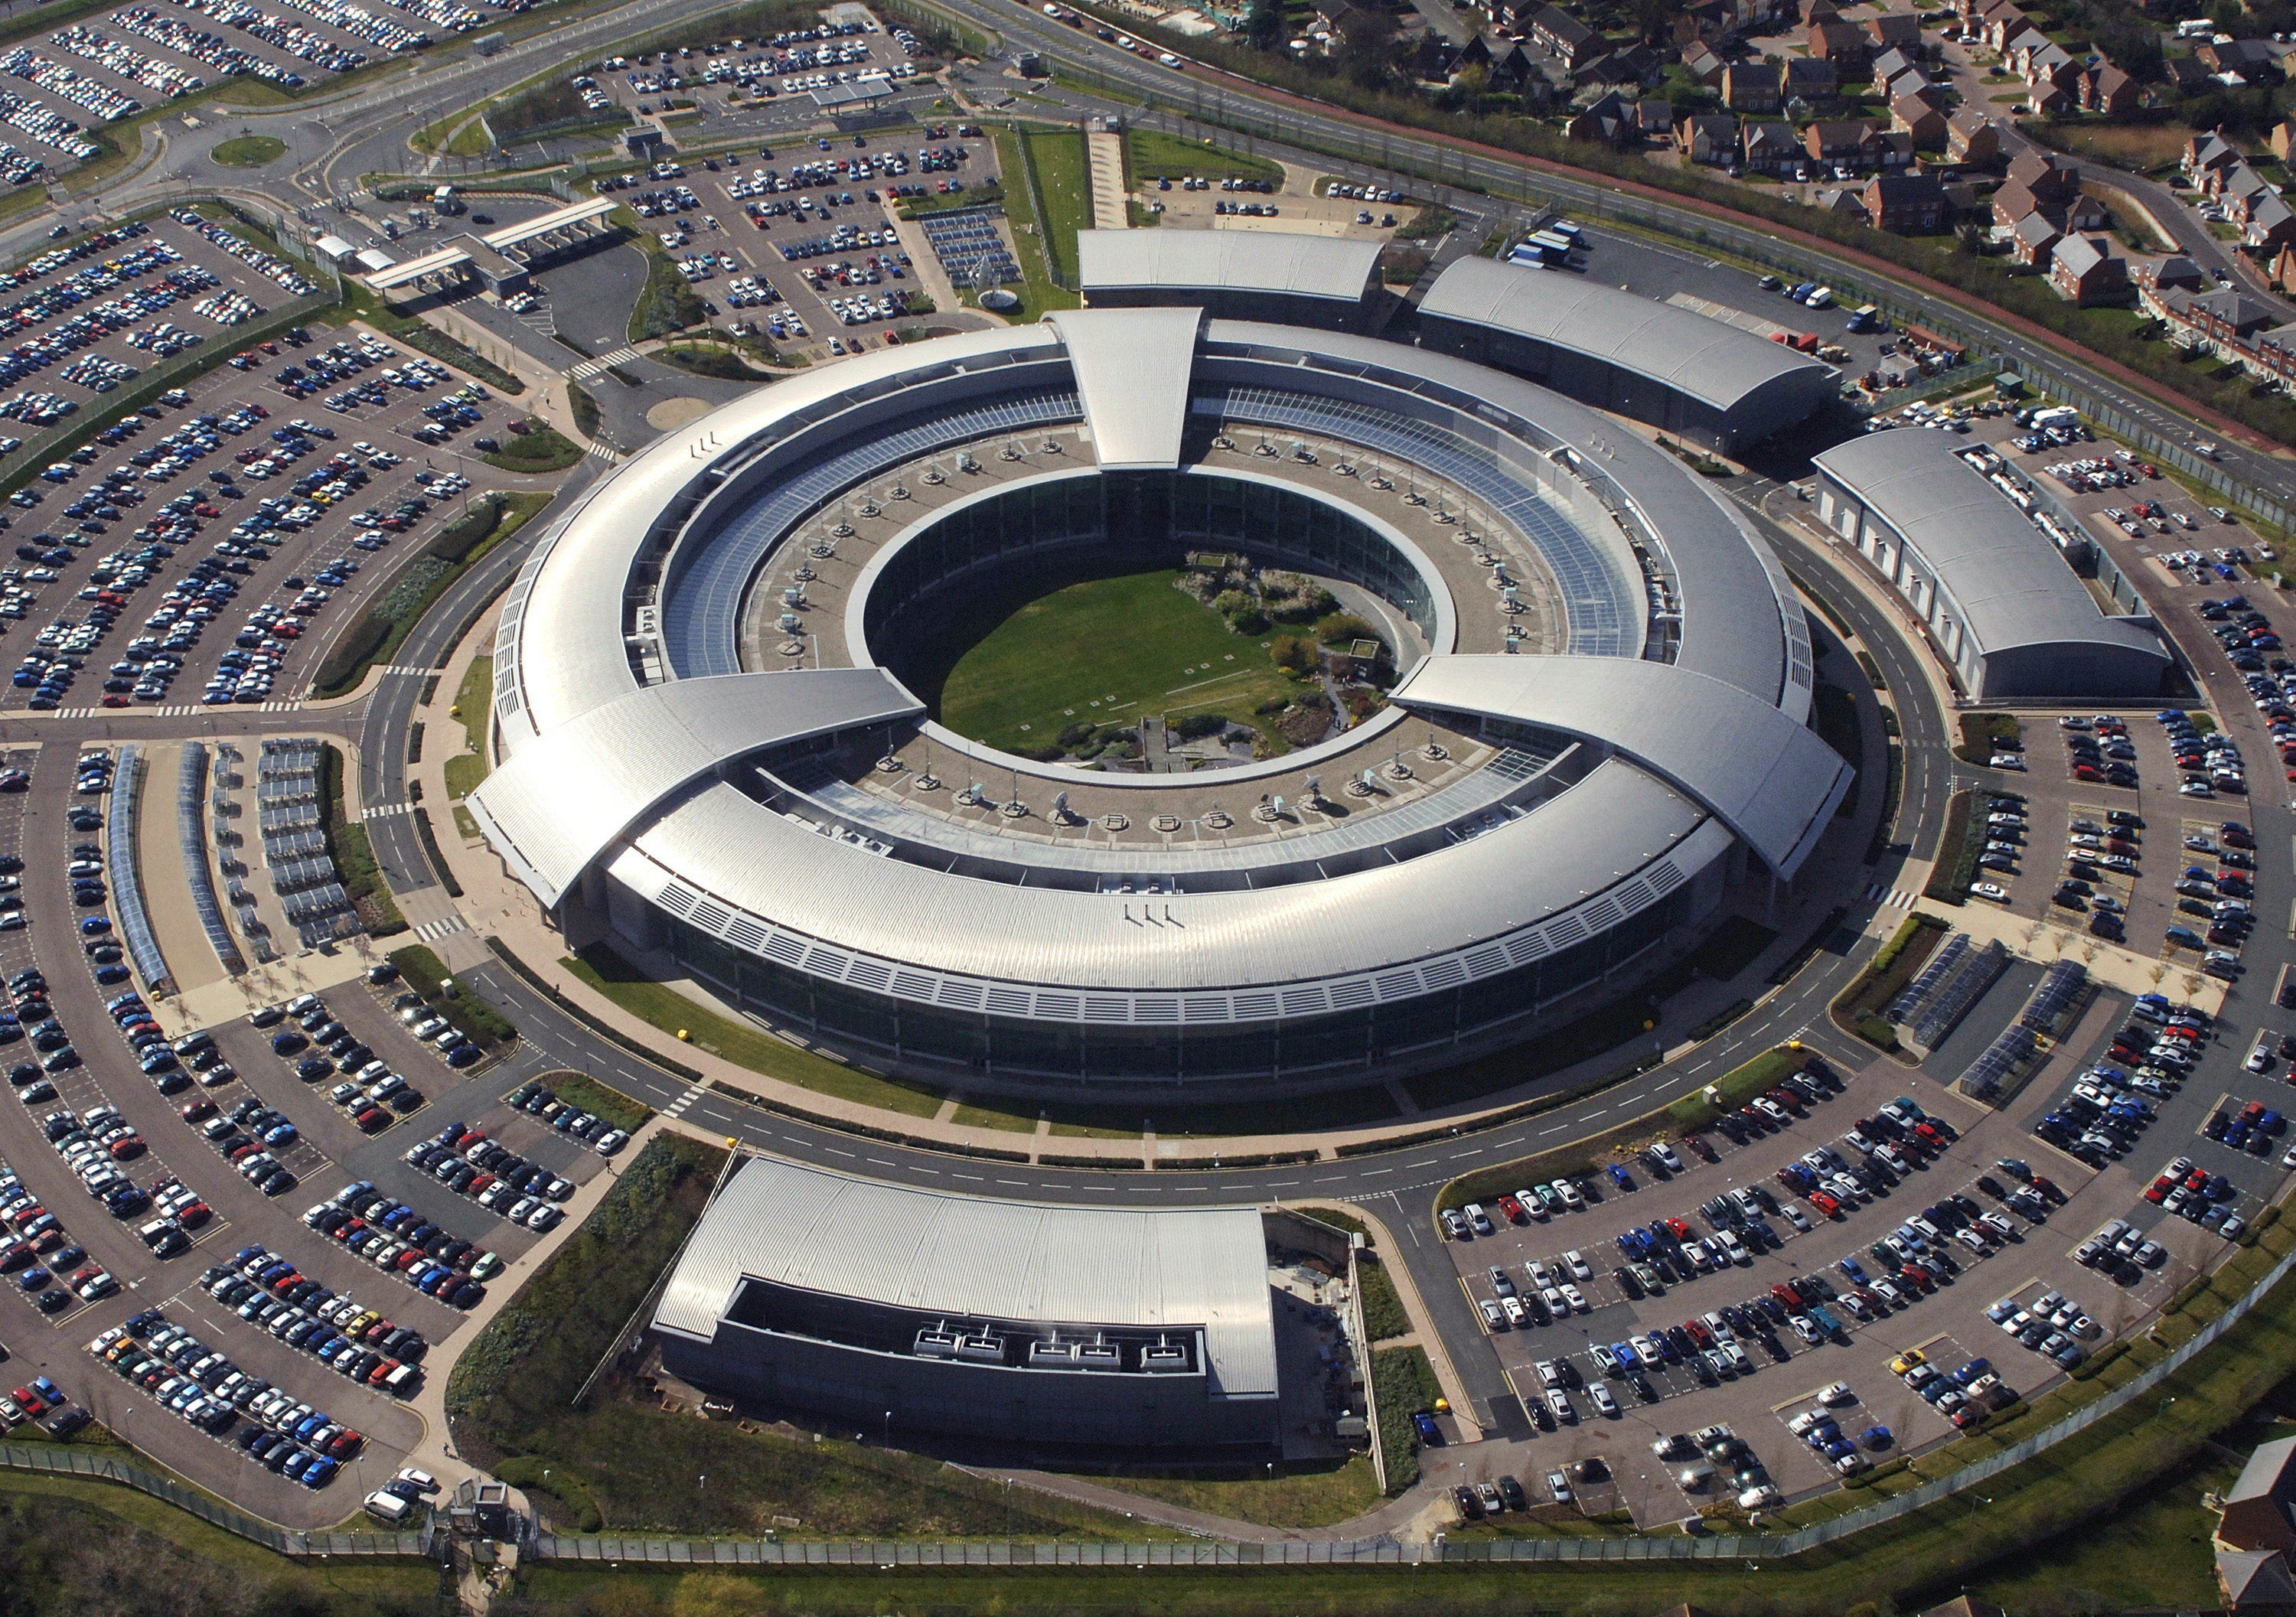
\includegraphics[scale=0.4]{gchq.jpg}
\caption[Les bureaux du GCHQ en photographie aérienne][6pt]{Les bureaux du GCHQ en photographie aérienne.}
\label{fig:gchq}
\end{figure}
\newpage
\newpage
\section{L'Allemagne et le BND}

\newthought{Le BND\footnote{Bundesnachrichtendienst} est} le service de
renseignement extérieur allemand, et le pendant technique de la NSA en
Allemagne. Les détails exacts de leur coopération ne sont pas tous connus, mais
on peut au moins citer quelques événements récents qui mettent en lumière des
liens de coopération étroits (bien que moins solides qu'avec le GCHQ).

\subsection{Opération EIKONAL}

\newthought{Il existe actuellement} très peu de détails techniques sur cette
opération, bien que de nombreux documents et témoignages soient venus récemment
(mai 2015) apporter un éclairage nouveau sur ce programme qui s'est déroulé entre 2004 et
2008.

\newthought{Ces nouveaux éléments} ont été apportés par les journaux allemands
Süddeutsche Zeitung\autocite{sudde}, NDR et WDR\autocite{NDR}, et montrent que la BND,
en partenariat avec Deutsche Telekom, a placé des équipements réseau (des
sondes, en l'occurrence) fournis par la NSA au sein du noeud d'échange (noeud
PoP) maintenu par l'opérateur allemand, à Francfort.

\vspace{0.7cm}
\begin{figure}
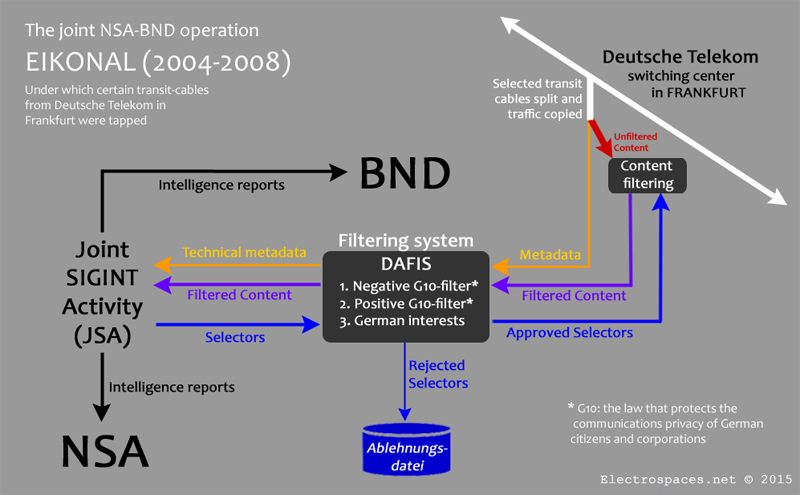
\includegraphics{eikonal1.jpg}
\caption[Architecture de l'opération EIKONAL][6pt]{Architecture
technique de l'opération}
\label{fig:eikonal1}
\end{figure}

\newthought{Ce schéma montre} l'organisation technique de l'opération : les
méta-données ainsi qu'une partie spécifique du trafic sont récupérées et passent
à travers un filtre nommé DAFIS\label{dafis}, qui sert à différencier les
communications provenant de citoyens allemands (que la BND n'a pas, légalement, le droit
d'espionner, de part son statut de service de renseignement \emph{extérieur}.
Dans ce cas de figure, elle doit passer par un <<~ordre G10~>> pour accéder
aux communications).
En fonction des résultats après passage dans le filtre, les données sont soit
renvoyés à la BND, soit directement à la NSA. Le schéma décisionnel est
reproduit ci-dessous :

\begin{figure}
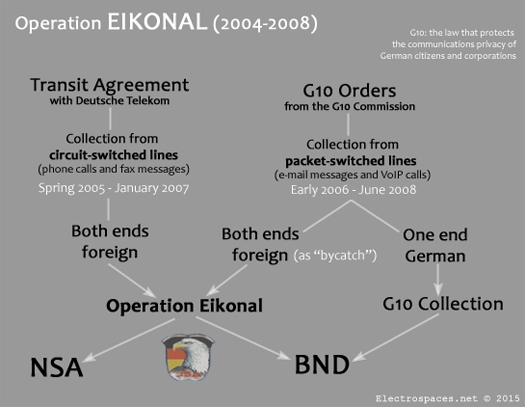
\includegraphics{eikonal2.jpg}
\caption[Schéma décisionnel de l'opération EIKONAL][6pt]{Schéma décisionnel}
\label{fig:eikonal2}
\end{figure}

\newthought{La mise sur écoute} concernait plus spécifiquement le câble FFM 21
reliant le Luxembourg et Francfort, contenant des canaux de fibres optiques
reliant le Luxembourg à Moscou, Prague, Vienne (où se trouvent des instances de
l'ONU) et Ankara\autocite{eikonal3}. Cela permettait à la NSA d'accéder à une partie du
monde auquel elle est très mal reliée directement.

\begin{figure}[!h]
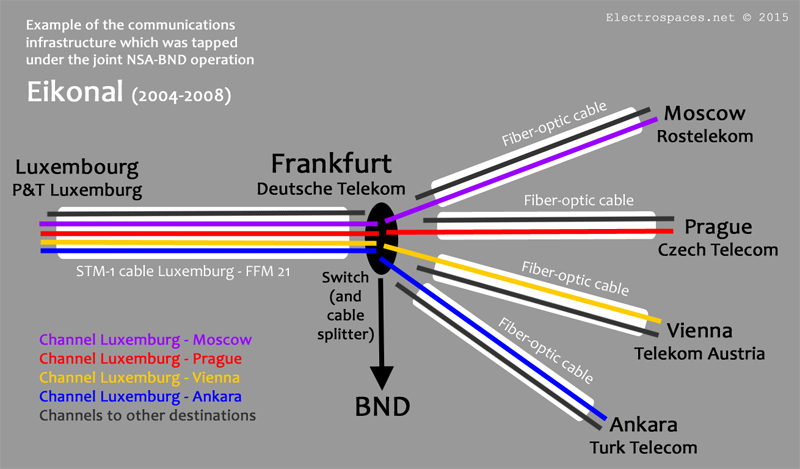
\includegraphics{eikonal3.jpg}
\caption[Schéma des canaux mis sur écoute][6pt]{Schéma des canaux mis sur
écoute}
\label{fig:eikonal3}
\end{figure}

\newpage
\newthought{EIKONAL a fait} parti d'un programme plus large de la NSA de
coopération avec des pays dits <<~tiers~>>, qui sont des pays ne faisant pas
partie de Five Eyes, mais qui coopèrent avec la NSA, de façon ponctuelle (comme
ici) ou de façon plus constante. Ce programme est nommé RAMPART-A, et concerne
un nombre inconnu de pays. L'Allemagne est connue pour en faire partie, alors
que de forts soupçons pèsent sur le Danemark\autocite{danemark} et qu'il est
rapporté, via des slides publiées par Snowden, qu'au moins cinq pays possèdent
des moyens similaires déployés sur leurs réseaux nationaux.

\begin{figure}
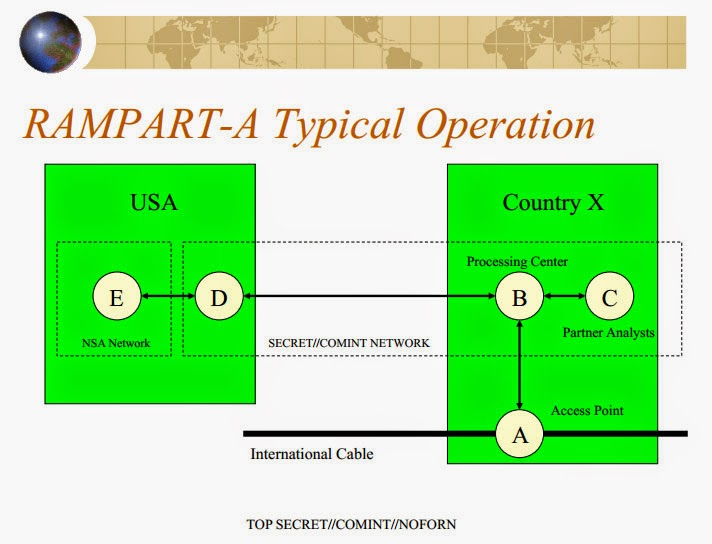
\includegraphics{rampart.jpg}
\caption[Schéma de l'opération RAMPART-A][6pt]{Schéma de l'opération RAMPART-A}
\label{fig:rampart}
\end{figure}


\newpage
\subsection{La station de Bad Aibling : nom de code GARLICK}

\begin{figure}
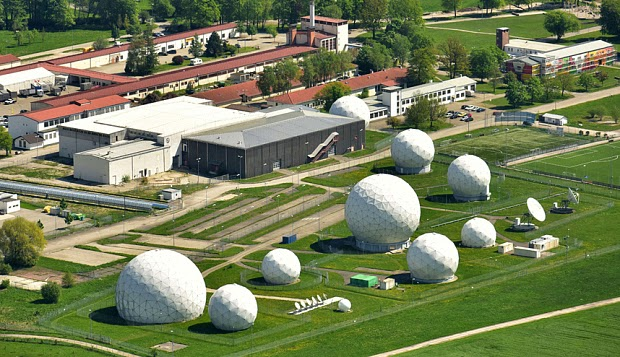
\includegraphics{ba1.jpg}
\caption[Station d'interception de Bad Aibling][6pt]{Station d'interception de
Bad Aibling, opérée par la BND à partir de 2004.}
\label{fig:ba1}
\end{figure}

\newthought{Cette station est} une ancienne station d'écoute du réseau ECHELON,
et appartenait anciennement à la NSA, qui l'a depuis rendue à l'Etat Fédéral en
2004 (tout en gardant une équipe opérationnelle sur le site).\autocite{spiegel}

\newthought{Il fut révélé} que la NSA pouvait accéder directement aux données
des interceptions, et fournissait même quatre des cinq listes de sélecteurs
utilisées pour savoir quoi chercher dans le flux de données (adresses IP,
numéros de téléphone, etc). 

\newthought{Initialement très petites}, c'est listes ce sont graduellement
remplies, au point que des contrôles manuels ne furent plus possibles. Elles
furent donc envoyées automatiquement plusieurs fois par semaine au siège de la
BND, où elles passaient à travers le DAFIS (voir page \pageref{dafis}) afin
d'exclure les communications impliquant des ressortissants ou citoyens
allemands, puis souvent renvoyées tel quel à la NSA.

\newthought{Ces sélecteurs furent} à l'origine d'un scandale à portée européenne
lorsqu'il fut révélé par certains médias allemands que ces listes contenaient
des entrées visant des employés du groupe Airbus\autocite{airbus}.

\newthought{Au total,} la collecte de méta-données, transmises directement à la
NSA après être passées par DAFIS, était de l'ordre de 200-220 millions par jour,
soit environ 6.6 milliards de méta-données collectées par mois\ldots\autocite{meta}


\begin{figure}
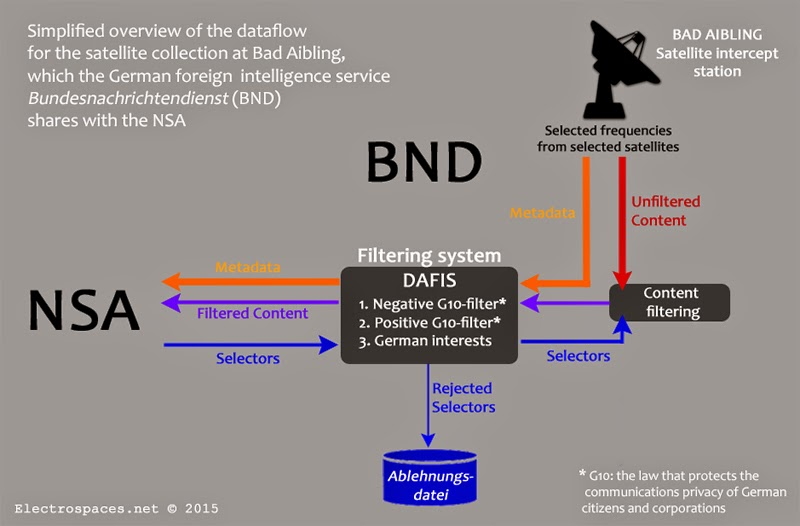
\includegraphics{ba2.jpg}
\caption[Schéma des interceptions à Bad Aibling][6pt]{Schéma des interceptions à Bad Aibling}
\label{fig:ba2}
\end{figure}


\begin{figure}
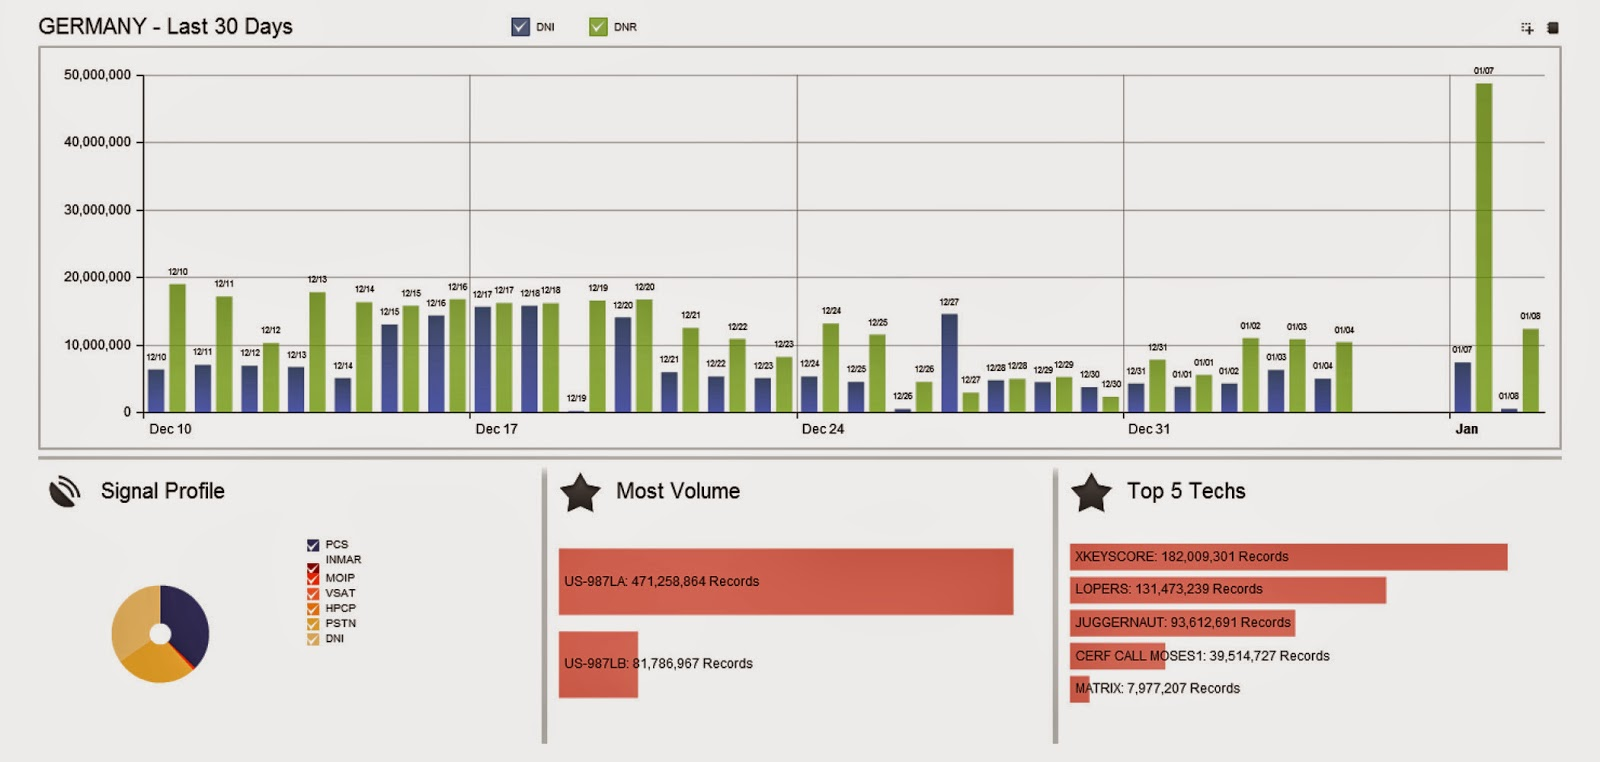
\includegraphics{ba3.jpg}
\caption[Capture écran de BOUNDLESSINFORMANT pour l'Allemagne][6pt]{552 millions
de meta-données entre décembre 2013 et janvier 2013\ldots}
\label{fig:ba3}
\end{figure}
\newpage
\newpage
\section{La France et la DGSE}

\newthought{La France a} elle aussi une longue tradition dans le chiffre, et ses
services de renseignement extérieur font partie des meilleurs du monde.
Contrairement au Royaume-Uni et à l'Allemagne, elle dispose de gros moyens
propres, et n'a donc pas une tradition de coopération avec la NSA aussi forte
que ses voisins. 

\newthought{En effet,} de part la présence d'un opérateur de catégorie mondiale
sur son territoire (Orange) ainsi que de différents points d'arrivées de câbles
sous-marins (Marseille pour le Proche-Orient notamment), la France est à un
carrefour stratégique des autoroutes numériques. La DGSE l'a bien compris, et
opère dans ses locaux parisiens le second plus gros programme de surveillance
européen, après celui des anglais\ldots\cite{DGSE}

\newthought{Pas franchement légal,} ce programme est soupçonné d'avoir été
complété par des installations\cite{reflets} d'équipements fournis par une
société \emph{française} spécialisée dans la technique dite de DPI\footnote{Deep
Packet Inspection :
l'analyse des flux de données en profondeur}, Amesys (filiale du géant français
Bull\ldots).
Cette dernière a fait l'objet d'une très longue saga d'articles publiés chez les journalistes d'investigation de
Reflets.info, et il n'est pas inutile d'aller lire la centaine de documents
publiés pour se rendre compte de la complexité de la chose.

\newthought{Il serait trop} long de faire un descriptif exhaustif des faits,
mais on peut retenir plusieurs choses :

\begin{itemize}
  \item Amesys a vendu un de ses produit d'interception de masse (au niveau
  d'un pays), EAGLE, au régime totalitaire de Kadhafi\cite{libye}
  \item Amesys est actuellement en train d'installer le même équipement au
  Maroc\cite{maroc}, ce qui inquiète fortement les opposants au régime
  marocain, déjà fortement réprimés.
  \item Qosmos, un autre leader du DPI et lui aussi français, a vendu des
  sondes d'inspection au régime de Bachar al-Assad en Syrie\cite{qosmos}
  \item Une plainte a été déposée par la FIDH pour << complicité de crimes de
  torture >> contre Qosmos et Amesys devant le Parquet de Paris.\cite{fidh}
\end{itemize}

\newthought{Ces faits sont} d'autant plus troublants que la société Elexo, soeur
d'Amesys, vient de candidater\cite{elexo} pour le marché public ouvert pour la
nouvelle Loi sur le Renseignement, votée il y a peu, et instaurant la mise en place de <<
boîtes noires >> sur les coeurs de réseau de l'Internet français\cite{LR} (du
DPI légal, en somme).

\newpage
\subsection{Frenchelon}

\newthought{Contraction des termes} <<~French~>> et <<~ECHELON~>>, ce nom
désigne les stations d'écoutes opérées sur le territoire national par la
DGSE\footnote{Direction Générale de la Sécurité Extérieure, les services secrets
français} et la DRM\footnote{Direction du Renseignement Militaire, la branche
en charge des renseignements au sein de l'Armée.}. Il en existerait une
quinzaine, dont la plus importante se situe à Domme :

\vspace{0.7cm}
\begin{figure}
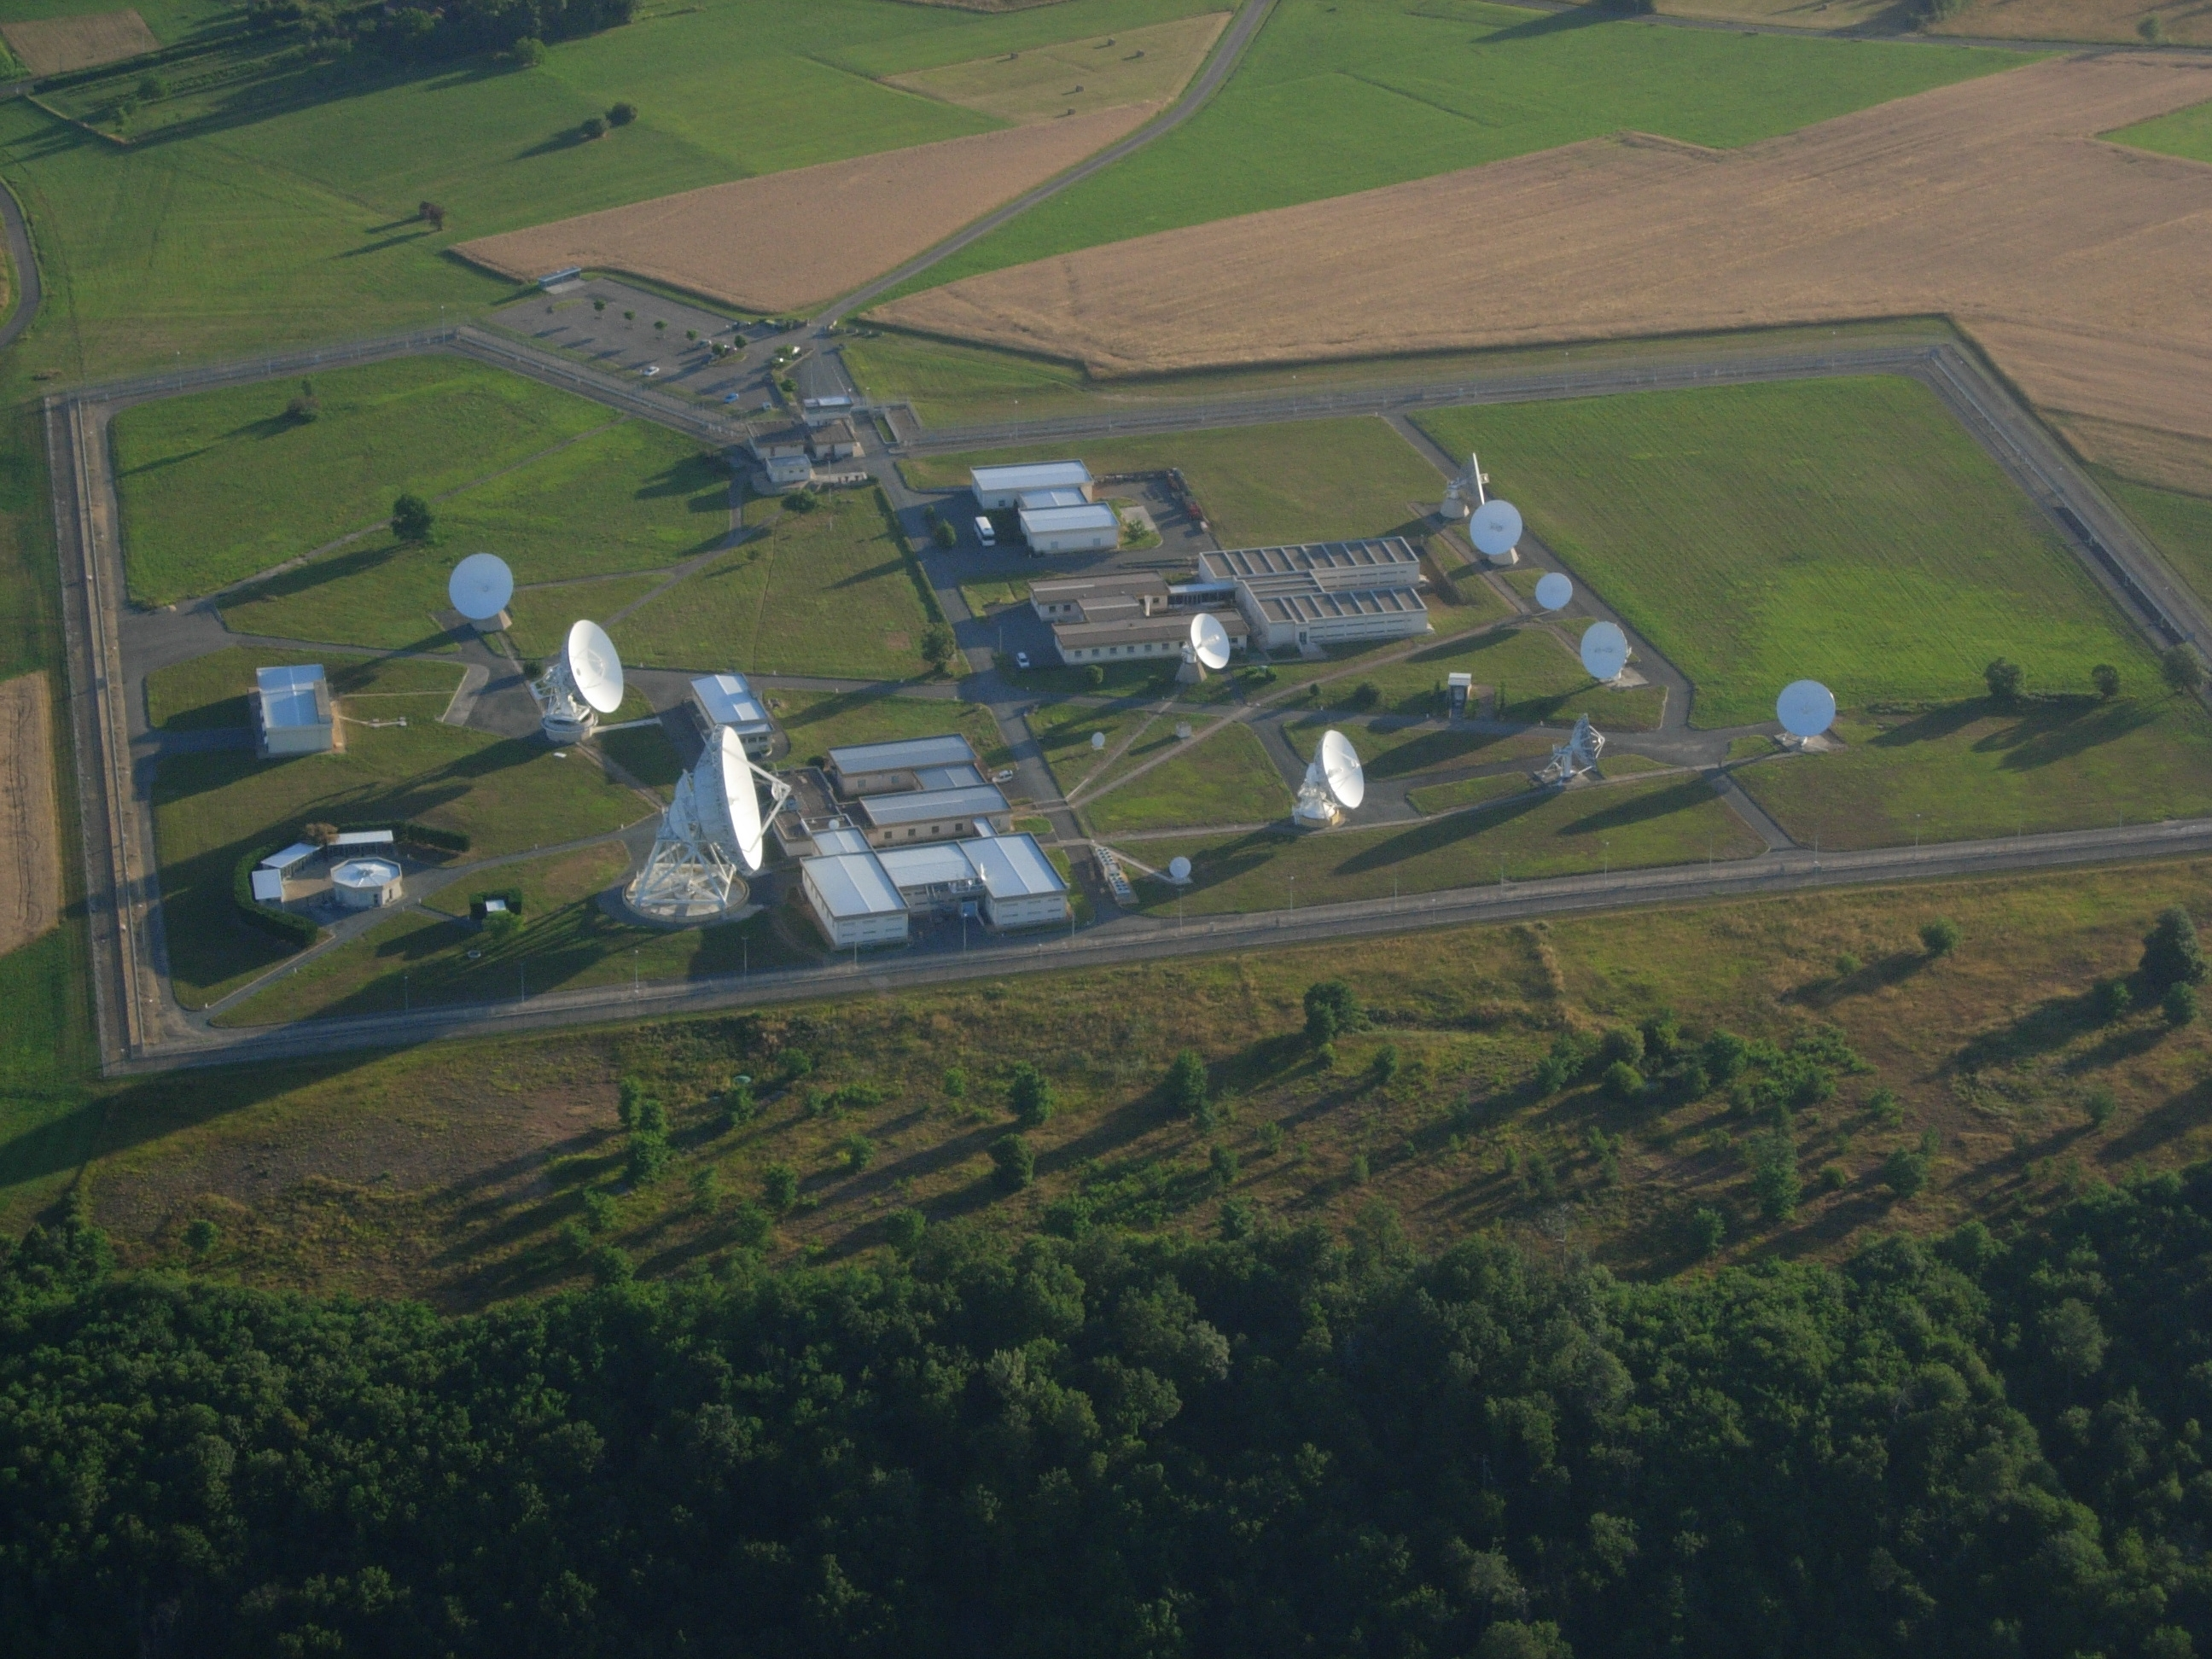
\includegraphics{french1.jpg}
\caption[Station d'écoute de Domme][6pt]{Station d'écoute de la DGSE
à Domme}
\label{fig:french1}
\end{figure}


\newthought{Tout comme ECHELON,} le programme français permet d'intercepter de
grandes quantités de données sur tout le spectre électromagnétique, afin d'être
analysées plus tard. Ces données peuvent être ensuite utilisées par tous les
acteurs du renseignement en France, et sont stockées dans les locaux parisiens
de la DGSE.\cite{bbf}

\newthought{Les technologies utilisées} par ce programme sont en partie issues
d'appels d'offres de la DGA et de développements assurés par EADS (aujourd'hui
Airbus Defence And Space), notamment le système HERISSON\footnote{Habile
extraction du renseignement d'intérêt stratégique à partir de sources ouvertes
numérisées}\cite{herisson} en charge de l'extraction de renseignements en
sources ouvertes (réseaux sociaux, Internet, etc).

\newpage
\subsection{L'accord LUSTRE}

\newthought{Derrière ce nom} se cache l'accord d'échange de données
interceptées signé entre la DGSE pour la partie française et la NSA pour la
partie américaine. C'est l'équivalent de l'accord UKUSA, mais contrairement à ce
dernier, très peu d'informations sont disponibles sur les modalités de l'accord.

\newthought{L'accord fut signé} fin 2011\cite{lustre}, et permet à la France
d'accéder aux données de la NSA sur des parties du monde où ses capacités de renseignement
sont limitées, tandis qu'elle fournit à la NSA des données sur lesquelles la
France dispose de bonnes connexions (voir figure \ref{fig:french2}), notamment
le Proche-Orient et l'Afrique (il y a environ trente fois plus de trafic Afrique -> Europe qu'Afrique ->
\EUA).

\vspace{0.7cm}
\begin{figure}
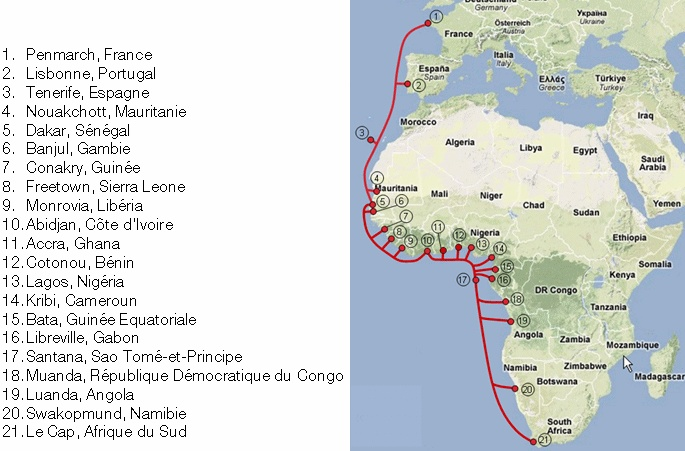
\includegraphics{french2.jpg}
\caption[Câble sous-marin reliant l'Afrique à l'Europe][6pt]{Câble sous-marin
reliant l'Afrique à l'Europe}
\label{fig:french2}
\end{figure}

\newthought{Ces informations expliquent} en partie le relatif silence des
autorités françaises à propos des révélations d'Edward Snowden, puisqu'elle se
permet de faire exactement la même chose de son côté. Il
est d'ailleurs intéressant de noter que l'accord LUSTRE fut révélé au public par
le Général Keith Alexander\footnote{La directeur de la NSA de l'époque} lors
d'une audition devant la commission de renseignement américaine, après que les pays
européens, dont la France, ont commencé à protester contre les révélations
faites sur PRISM. Faites ce que je dis\ldots


%------------------------------------------------


%------------------------------------------------
